\documentclass[tikz,border=4pt]{standalone}
% Paleta y fuentes compartidas por el libro y las figuras (única fuente de verdad).
\RequirePackage{xcolor}
\definecolor{oxido}{HTML}{B7410E}
\definecolor{cobre}{HTML}{D27D2D}
\definecolor{carbon}{HTML}{2B2B2B}
\definecolor{azul}{HTML}{1F5F8B}
\definecolor{arena}{HTML}{F4EDE4}

\usepackage{fontspec}
\setsansfont{FiraSans}[Extension=.otf,UprightFont=*-Regular,BoldFont=*-SemiBold,ItalicFont=*-Italic,BoldItalicFont=*-SemiBoldItalic]
\setmonofont{FiraMono}[Extension=.otf,UprightFont=*-Regular,BoldFont=*-Medium,Scale=0.95]
\usetikzlibrary{positioning,arrows.meta,calc,decorations.pathreplacing}
\begin{document}
\sffamily\small
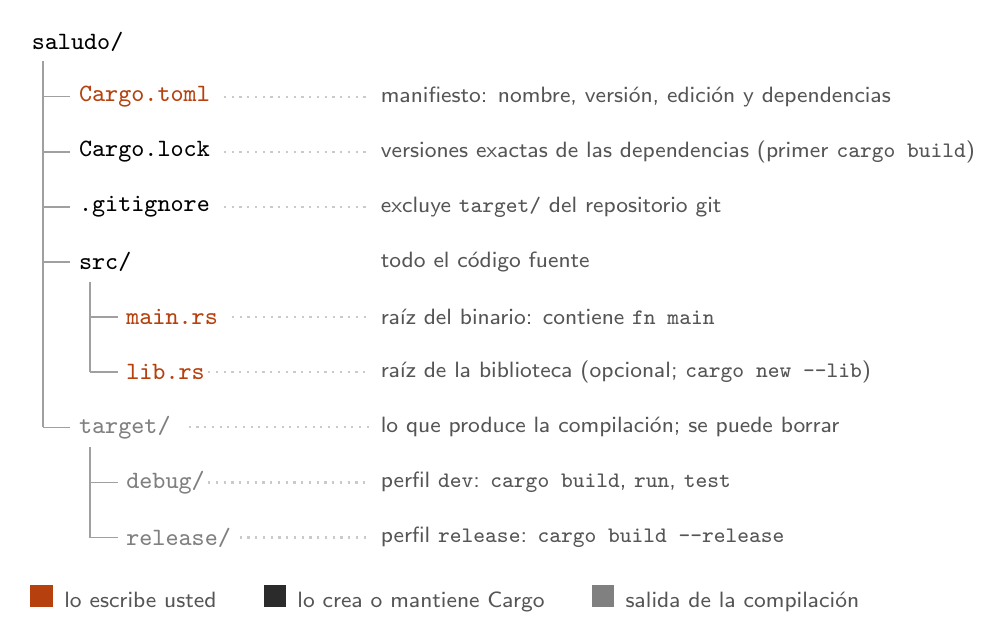
\begin{tikzpicture}[>={Stealth[length=2.2mm]},
  archivo/.style={anchor=west,font=\ttfamily\small,inner sep=1.5pt},
  nota/.style={anchor=west,font=\sffamily\footnotesize,text=carbon!80,inner sep=1pt},
  rama/.style={draw=carbon!45,line width=0.6pt}]
  % Filas: y = -0.7 * i
  \def\paso{0.7}
  % Árbol (líneas)
  \draw[rama] (0.15,-0.25) -- (0.15,-6*\paso);
  \foreach \i in {1,2,3,4,7} {\draw[rama] (0.15,-\i*\paso) -- (0.5,-\i*\paso);}
  \draw[rama] (0.75,-4*\paso-0.25) -- (0.75,-6*\paso);
  \foreach \i in {5,6} {\draw[rama] (0.75,-\i*\paso) -- (1.1,-\i*\paso);}
  \draw[rama] (0.15,-6*\paso) -- (0.15,-7*\paso);
  \draw[rama] (0.75,-7*\paso-0.25) -- (0.75,-9*\paso);
  \foreach \i in {8,9} {\draw[rama] (0.75,-\i*\paso) -- (1.1,-\i*\paso);}
  % Nombres
  \node[archivo,font=\ttfamily\small\bfseries] at (-0.05,0) {saludo/};
  \node[archivo,text=oxido] at (0.55,-1*\paso) {Cargo.toml};
  \node[archivo] at (0.55,-2*\paso) {Cargo.lock};
  \node[archivo] at (0.55,-3*\paso) {.gitignore};
  \node[archivo,font=\ttfamily\small\bfseries] at (0.55,-4*\paso) {src/};
  \node[archivo,text=oxido] at (1.15,-5*\paso) {main.rs};
  \node[archivo,text=oxido] at (1.15,-6*\paso) {lib.rs};
  \node[archivo,font=\ttfamily\small\bfseries,text=carbon!60] at (0.55,-7*\paso) {target/};
  \node[archivo,text=carbon!60] at (1.15,-8*\paso) {debug/};
  \node[archivo,text=carbon!60] at (1.15,-9*\paso) {release/};
  % Guías punteadas y notas
  \foreach \i/\x in {1/2.45,2/2.45,3/2.45,5/2.55,6/2.25,8/2.25,9/2.65} {
    \draw[carbon!25,dotted,line width=0.8pt] (\x,-\i*\paso) -- (4.3,-\i*\paso);}
  \draw[carbon!25,dotted,line width=0.8pt] (2.0,-7*\paso) -- (4.3,-7*\paso);
  \node[nota] at (4.4,-1*\paso) {manifiesto: nombre, versión, edición y dependencias};
  \node[nota] at (4.4,-2*\paso) {versiones exactas de las dependencias (primer \texttt{cargo build})};
  \node[nota] at (4.4,-3*\paso) {excluye \texttt{target/} del repositorio git};
  \node[nota] at (4.4,-4*\paso) {todo el código fuente};
  \node[nota] at (4.4,-5*\paso) {raíz del binario: contiene \texttt{fn main}};
  \node[nota] at (4.4,-6*\paso) {raíz de la biblioteca (opcional; \texttt{cargo new -{}-lib})};
  \node[nota] at (4.4,-7*\paso) {lo que produce la compilación; se puede borrar};
  \node[nota] at (4.4,-8*\paso) {perfil \texttt{dev}: \texttt{cargo build}, \texttt{run}, \texttt{test}};
  \node[nota] at (4.4,-9*\paso) {perfil \texttt{release}: \texttt{cargo build -{}-release}};
  % Leyenda
  \node[nota] at (-0.05,-10.1*\paso) {\textcolor{oxido}{\rule{8pt}{8pt}}\, lo escribe usted\qquad
    \textcolor{carbon}{\rule{8pt}{8pt}}\, lo crea o mantiene Cargo\qquad
    \textcolor{carbon!60}{\rule{8pt}{8pt}}\, salida de la compilación};
\end{tikzpicture}
\end{document}
